
This chapter will give information on the classification method called k-Nearest Neighbour (k-NN).

The NN is shortly "given a collection of data point and query points in an m-dimensional metric space, find the data point that is closets to the query point"
\citep{meaningfulNN}.
\section{Classification using Nearest Neighbour}

\begin{figure}[h]
	\begin{center}
		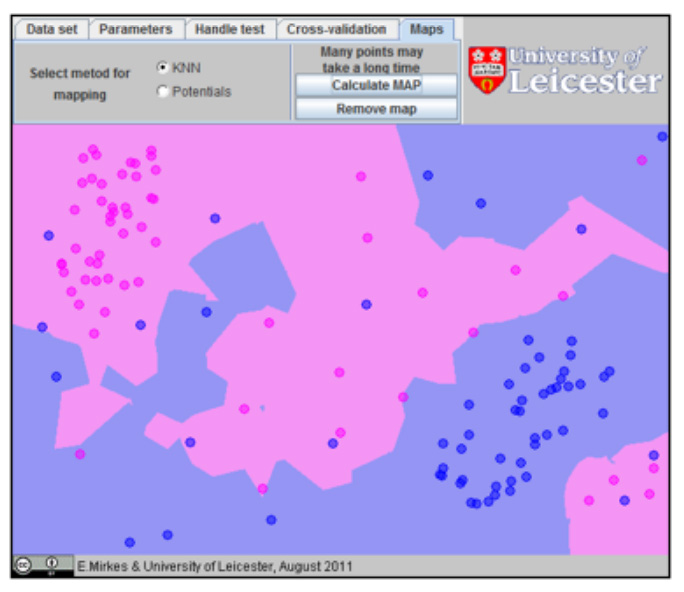
\includegraphics[scale = 0.5]{fig/KNNfig.jpg}
		\caption{Illustration of how k-NN will divide the space up with to different classes \citep{introKNN}}
		\label{KNN fig}
	\end{center}
\end{figure}
This means that the NN classification will need a dataset that can train a system \citep{Sinyor05}, the data used for training has to be annotated so that the program that makes the classification 'knows' what the different data represent. Practically, this is just calculating feature vectors for all, in this case, sounds, and saving them for testing.

When a test-sound is to be classified, a feature vector is calculated using the same features and feature parameters as used when training the k-NN.
The euclidean distance is then calculated between the test-feature vector and all the train-feature vectors \citep{NNHD}.
The k is the amount of neighbours that will be considered when classifying a test-feature vector. The class of the majority of the k nearest neighbours will then be the most represented sound, and thus the input will be labelled as that class\citep{introKNN}.

\begin{figure}[h]
	\begin{center}
	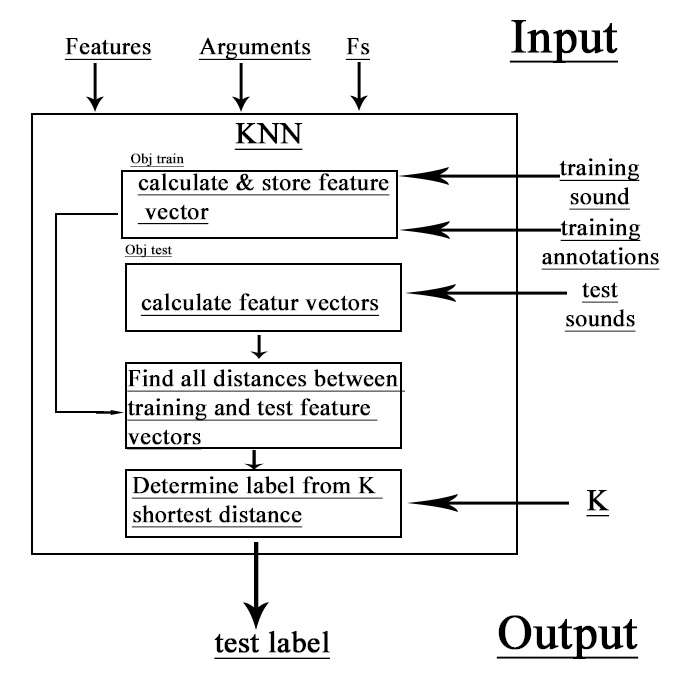
\includegraphics[scale=0.5]{fig/diagram2.jpg}
	\caption{Flowchart of our KNN implementation}
	\label{KNN:flow}
	\end{center}
\end{figure}

Our implementation is created as a Matlab class, as to ease future changes and/or development. 
